\subsection{Surface temperature gradients}

\begin{figure}[H]
	\centering
	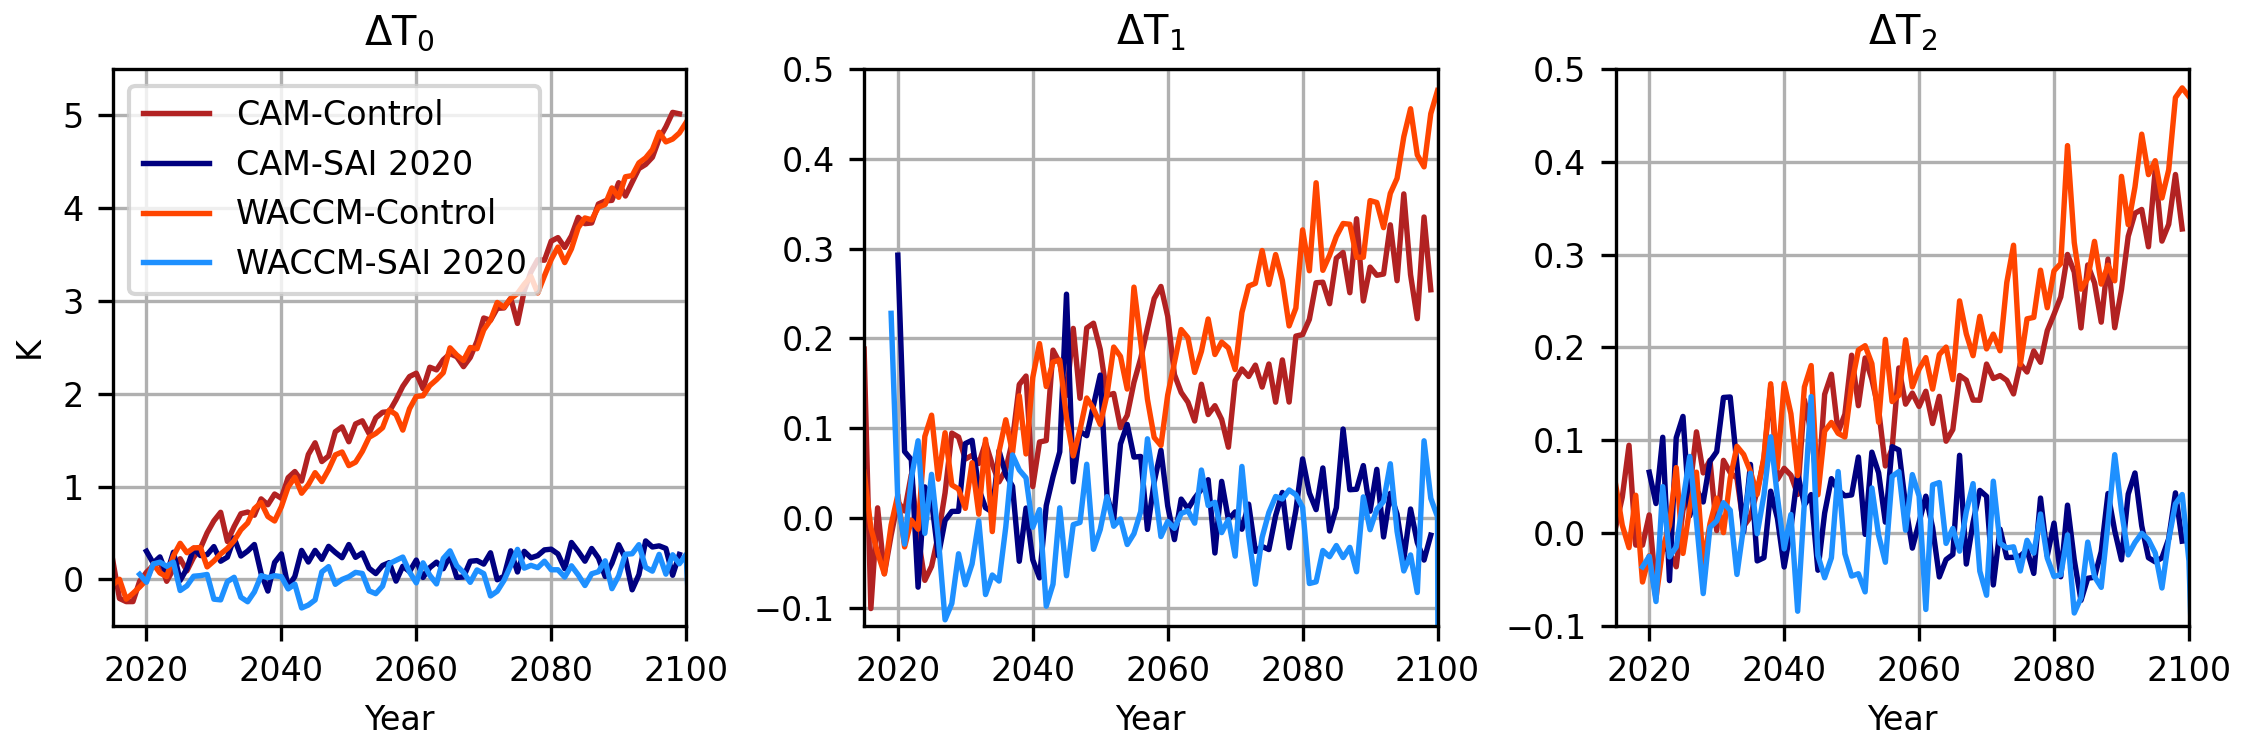
\includegraphics[width=\linewidth]{/Users/Simone/Documents/Uni/Master/Y2/Thesis/Paper_imgs/png/Tgrad_2.png}
	\caption{Temperature gradients $T_0$, $T_1$, $T_2$ as compared to 2016-2025 mean, for Control and SAI2020 scenarios in CAM and WACCM}
	\label{fig:Tgrad}
\end{figure}

The surface temperature gradients as described by Kravitz et al. are shown in Figure \ref{fig:Tgrad}, we learn:
\begin{itemize}
	\item The global mean surface temperature $T_0$ is very comparable in both scenarios between the models.
	\item Early century CAM-SAI2020 might be slightly higher, but in later century shows very similar behaviour to WACCM-SAI2020.
	\item Pole-to-pole gradient $T_1$ shows similar behaviour in the first few years, both WACCM and CAM show a clear increase compared to control after initialisation, followed by a stark drop down to reference levels. 
	\item Early-mid century CAM-SAI2020 possibly more variability compared to WACCM-SAI2020, late century very similar.
	\item -> expected because the earosol field was taken from late century.
	\item Inter-hemispheric temperature $T_2$ also shows very similar behaviour in both scenarios. 
	\item possibly more variability in early century CAM-SAI2020 compared to WACCM-SAI2020, but both seem to show a decrease in variabilty in late century. 
\end{itemize}

TO DO:
\begin{itemize}
	\item Apply some statistical analysis on these sets? Or is qualitative analasys enough? Maybe running mean and standard deviation? nah
	\item titels ipv y-labels maken 
\end{itemize}